\section{CPU Virtual}

\Glspl{so} convidados não possuem conhecimento dos núcleos físicos do processador da plataforma.
Por isso, grande parte dos hipervisores, incluindo este, implementa o conceito de CPUs virtuais, que simulam na prática um núcleo físico do processador.
Dessa forma, para cada CPU de uma \gls{vm}, cria-se uma \textit{thread} encarregada de simular a execução de código do núcleo.

Além da execução de código, as CPUs virtuais também são responsáveis por redirecionar eventos às suas respectivas \glspl{vm}.
Como existe um mapeamento um para um entre \textit{threads} e CPUs virtuais, quando ocorre um evento, é possível verificar o ponteiro da CPU virtual em execução naquele instante e, por meio dela,
identificar a \gls{vm} correspondente.

\begin{figure}[H]
\centering
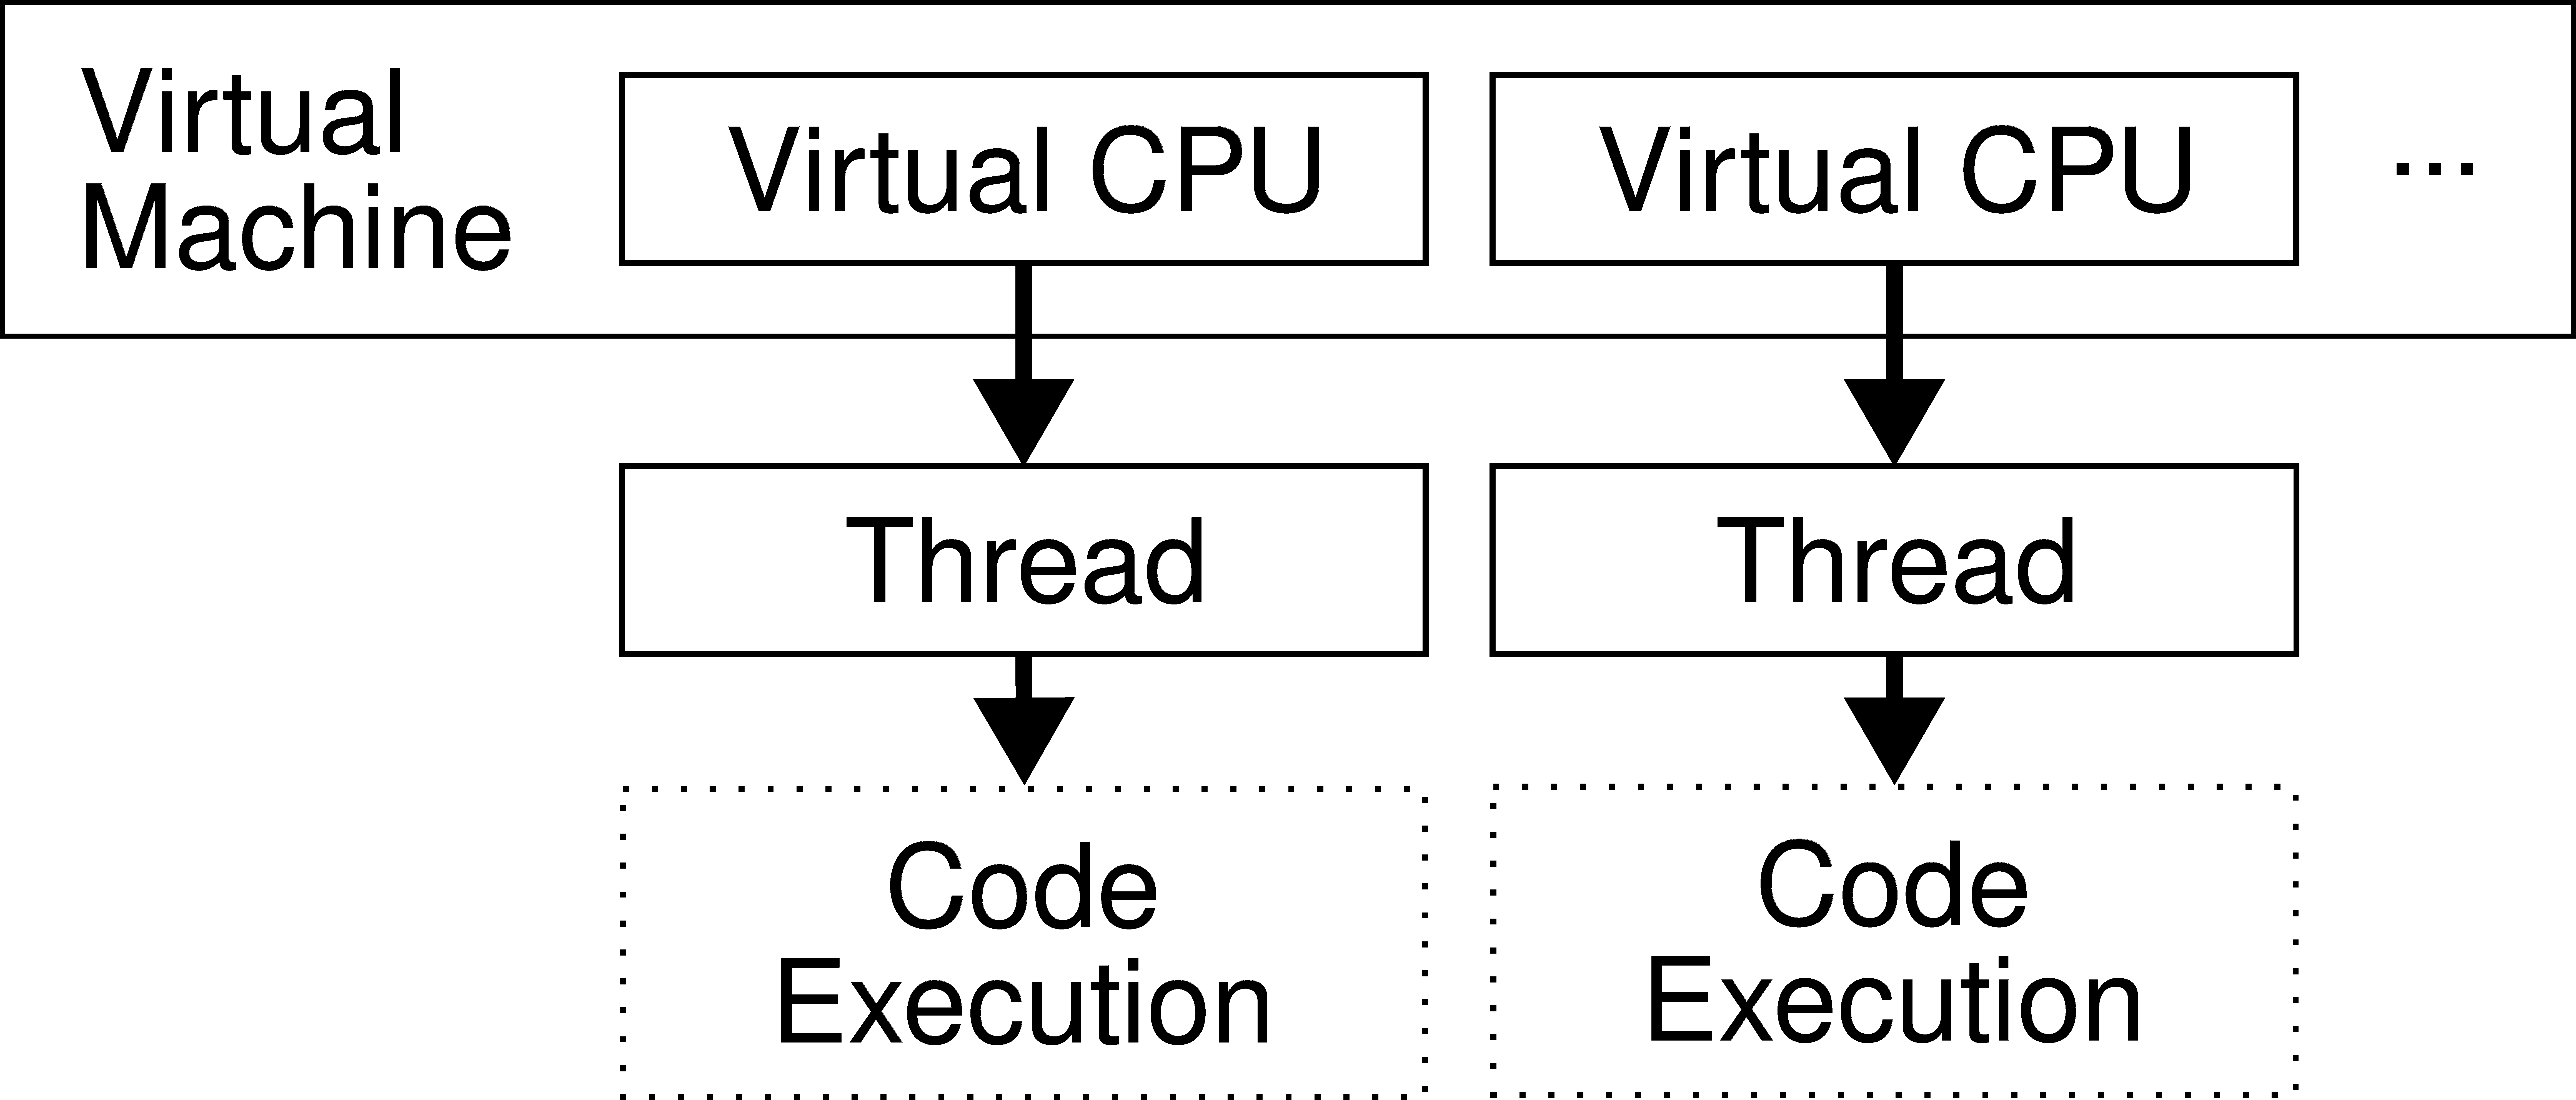
\includegraphics[width=0.6\textwidth]{images/VirtualCPUsToThreads.pdf}
\caption{Diagrama de Mapeamento de CPUs Virtuais Para Threads}\label{fig:virtual-cpus-to-threads}
\end{figure}
